\chapter{Cellular Automata}

Cellular Automata (CA) are parallel computing models, whose evolution
is ruled by local rules. A cellular automaton can be thought as a
$d$-dimensional space, the \emph{cellular space}, subdivided in
regular cells of uniform shape and size. Each cell embeds a
\emph{finite automaton}, that is one of the most simple and well known
computational model in Computer Science and can assume a finite number
of states. At time $t=0$, cells are in arbitrary states and the CA
evolves step by step by changing the states of the cells at discrete
time steps, by applying the same local rule of evolution, i.e. the
cell's \emph{transition function}, simultaneously (i.e. in parallel)
to each cell of the CA. Input for the cell is given by the states of a
predefined set of neighboring cells, which is assumed constant in
space and time.

It is possible to indentify an informal definition of cellular
automaton by simply listing it main properties:

\begin{itemize}
\item It is formed by a $d$-dimensional space, called \emph{cellular
  space}, partitioned into cells of uniform shape (triangles, squared,
  hexagons, cubes) and size (see Figure \ref{fig:CellularSpaces});
\item The number of cell states is finite;
\item The evolution occurs through discrete steps;
\item Each cell evolves by simultaneously changing its state by
  applying the same transition function to the cellular space;
\item The transition function depends on the state of the central and
  neighboring cells
\item The relationship of closeness that defines the neighborhood of a
  cell is local, uniform and invariant over time.
\end{itemize}

\begin{figure}
  \begin{center}
    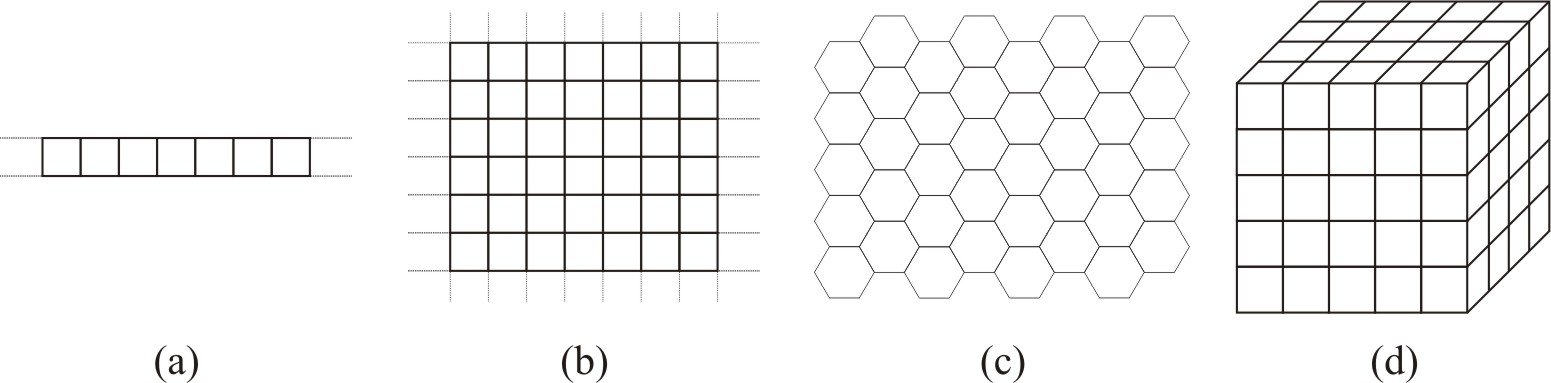
\includegraphics[width=12cm]{./images/CellularAutomata/CellularSpaces}
    \caption{Example of cellular spaces: (a) one-dimensional, (b)
      two-dimensional with square cells, (c) two-dimensional with
      hexagonal cells, (d) three-dimensional with cubic cells.}
    \label{fig:CellularSpaces}
  \end{center}
\end{figure}

The cell's relationship of closeness depends on the geometry. 

Despite their simple definition, CA can exhibit very interesting,
complex global behaviors. Moreover, from a computational point of
view, they are equivalent to Turing Machines. CA are particularly
adapt to model and simulate complex systems, i.e. those systems
characterized by interaction of numerous elementary constituents. As a
matter of fact, they have been largely employed different scientific fields.

